\documentclass{article}
\usepackage[utf8]{inputenc}
\usepackage{titling}
\usepackage{graphicx}
\usepackage{xcolor}
\usepackage[colorlinks=true,linkcolor=darkgray]{hyperref}
\usepackage[spanish]{babel}


\title{PRÁCTICA 7: TLS}
\author{Cristina Díaz García}
\date{Enero 2019}

\renewcommand\maketitlehooka{\null\mbox{}\vfill}
\renewcommand\maketitlehookd{\vfill\null}


\begin{document}

\addcontentsline{toc}{section}{Índice general}

\begin{titlingpage}
\maketitle
\end{titlingpage}

\newpage

\tableofcontents

\newpage

\section{Ejercicio 1}

\textbf{\textit{https://www.meneame.net}}

\begin{flushleft}
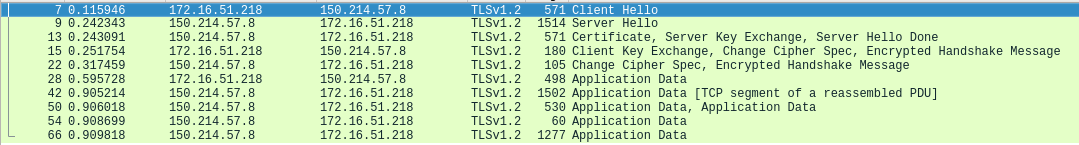
\includegraphics[scale=0.4]{meneame.png}
\end{flushleft}

\textbf{\textit{https://tls13.pinterjann.is/}}

\begin{flushleft}
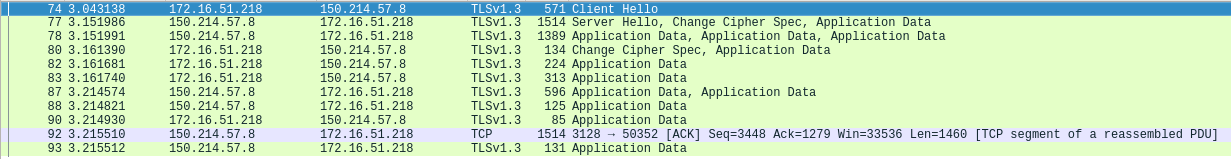
\includegraphics[scale=0.35]{tls13.png}
\end{flushleft}

\begin{itemize}
\item ¿Cuándo se procede con el handshake y la fase de conexión?

En ambos casos se inicia con el Client Hello que se envía al abrir la página.

En el caso de \textit{https://www.meneame.net}, esto ocurre en el séptimo paquete. Con \textit{https://tls13.pinterjann.is/}, es en el número 74.
\item ¿Qué versión de TLS se utiliza?

En el caso de \textit{https://www.meneame.net}, se usa la versión 1.2 de TLS. Por otra parte, \textit{https://tls13.pinterjann.is/} usa la 1.3.
\item En la parte del cliente, ¿en qué trama se puede ver la suite de cifrado? ¿Cómo se interpreta la suite de cifrado?

En la capa de Secure Sockets Layer (SSL).

\begin{center}
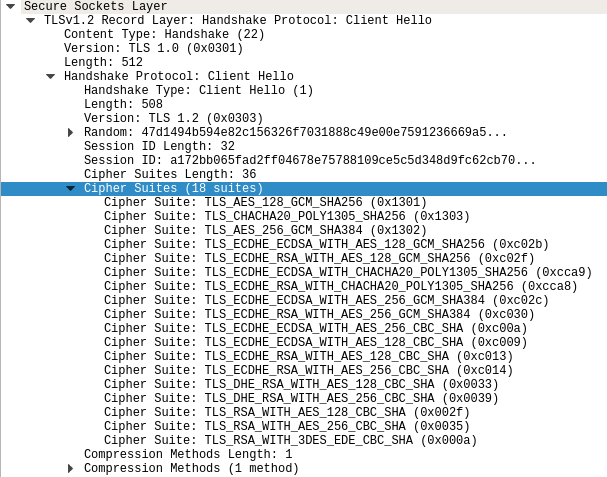
\includegraphics[scale=0.4]{suites.png}
\end{center}

\begin{center}
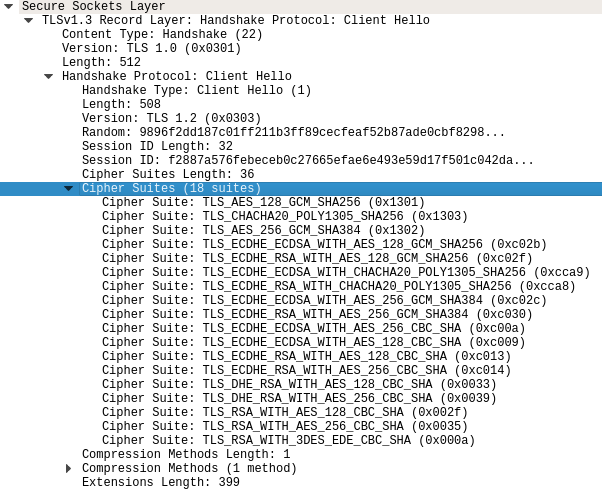
\includegraphics[scale=0.35]{suites2.png}
\end{center}

Se interpreta como los protocolos y algoritmos que se usan para proteger la información: se usa TLS, opcionalmente un algoritmo de intercambio de clave (RSA, Diffie-Hellman efímero, curvas elípticas...), el algoritmo de cifrado y los modos en los que trabaja (AES128, 3DES\_CBC, CHACHA20...) y finalmente la función que usa para el Hash (SHA256, SHA384...)
\item ¿Qué suite de cifrado se acepta finalmente para el proceso de conexión?

\begin{center}
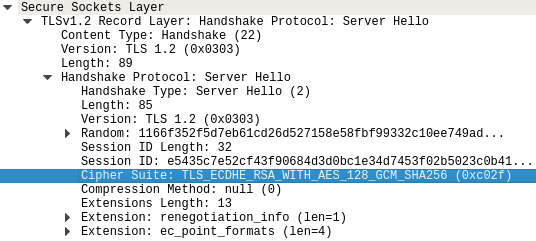
\includegraphics[scale=0.4]{suite.png}
\end{center}

\begin{center}
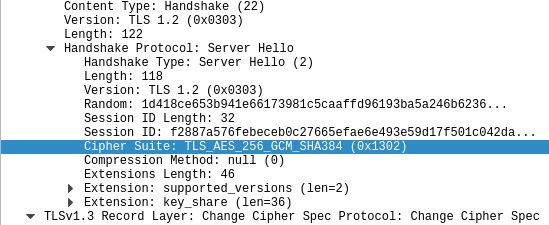
\includegraphics[scale=0.35]{suite2.png}
\end{center}

En el caso de \textit{https://www.meneame.net}, finalmente se usa \\TLS\_ECDHE\_RSA\_WITH\_AES\_128\_GCM\_SHA256. Por otra parte, \textit{https://tls13.pinterjann.is/} usa TLS\_AES\_256\_GCM\_SHA384.
\item ¿En qué trama se envía el certificado digital del servidor? \\ \underline{NOTA: No responder esta pregunta para la web (b)}

En la número 13.

\begin{center}
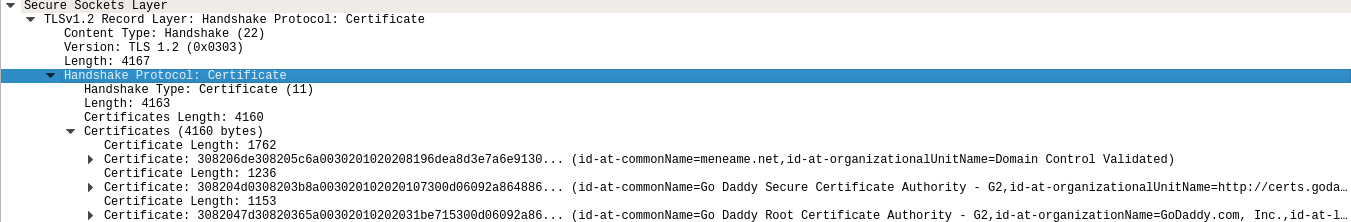
\includegraphics[scale=0.3]{certificate.png}
\end{center}
\item ¿El servidor se autentica al cliente? ¿Y el cliente al servidor?

El servidor se autentica mediante el paso del certificado digital (apartado anterior). El cliente en ningún momento se autentica.
\end{itemize}

\newpage

\section{Ejercicio 2}

\begin{itemize}
\item Explica con tus palabras cual es la principal diferencia entre TLS v1.2 y TLS v1.3 desde el punto de vista del handshake inicial.

\textbf{TLS v1.2}

\begin{flushleft}
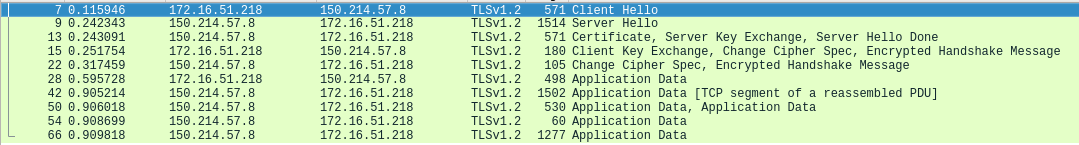
\includegraphics[scale=0.4]{meneame.png}
\end{flushleft}

\textbf{TLS v1.3}

\begin{flushleft}
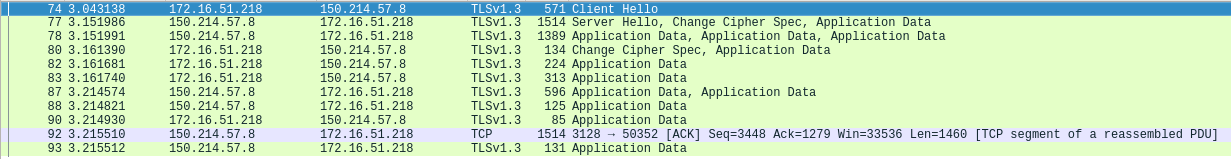
\includegraphics[scale=0.35]{tls13.png}
\end{flushleft}

Como se puede ver, en el primer mensaje del servidor, \textit{Server Hello}, se envía también la activación de la suite (\textit{Change Cipher Spec}), por lo que el inicio de las comuncaciones se hace más rápidamente.

También se intercambian las claves al inicio de la sesión, lo que permite empezar a cifrar desde el principio, que lleva también a una mayor rapidez y seguridad de la comunicaicón.
\item ¿En qué momento se envía el certificado digital del servidor?

En el mismo momento en el que se pasa el \textit{Server Hello}. Va cifrado porque las claves ya se habían intercambiado previamente.
\end{itemize}

\end{document}